% % % % % % % % % % % % % % % % % % % % % % % % % % % % % % % %
% import configuration
% % % % % % % % % % % % % % % % % % % % % % % % % % % % % % % %

% % % % % % % % % % % % % % % % % % % % % % % % % % % % % % % %
% Konfiguration
% % % % % % % % % % % % % % % % % % % % % % % % % % % % % % % %
\newcommand{\titleinfo}{Pflichtenheft}
\newcommand{\subjectinfo}{Projektname}
\newcommand{\authorinfo}{Michael Trummer}
\newcommand{\versioninfo}{0.1}
\newcommand{\docNr}{ABC.0001}
\newcommand{\dateinfo}{01.03.2017}

% Notes for SRS completion, uncomment the following command to suppress this output
\newcommand{\note}[1]{%
    \vspace{0.25cm}%
    \colorbox{grey}{%
        \parbox{\linewidth-6pt}{%
            \vspace{0.5cm}%
            \centering%
            \parbox{\linewidth-1cm}{%
                \footnotesize{#1}%
            }%
            \vspace{0.5cm}%
        }%
    }%
    \vspace{0.25cm}}
%\newcommand{\note}[1]{}

% % % % % % % % % % % % % % % % % % % % % % % % % % % % % % % %
% Packages, Layout, Units, etc.
% % % % % % % % % % % % % % % % % % % % % % % % % % % % % % % %
%%%%%%%%%%%%%%%%%%%%%%%%%%%%%%%%%%%%%%%%%%
% Dokument
%%%%%%%%%%%%%%%%%%%%%%%%%%%%%%%%%%%%%%%%%%
% Geometrie
\newcommand{\paperFormat}{a4paper}
\newcommand{\lPageMargin}{20mm}
\newcommand{\rPageMargin}{20mm}
\newcommand{\tPageMargin}{20mm}
\newcommand{\bPageMargin}{20mm}

\documentclass[11pt,oneside]{scrartcl}

\newcommand{\newpar}{\par\par}

\usepackage[pdftitle={\titleinfo},%
			pdfauthor={\authorinfo},%
			pdfcreator={pdfLatex, LaTeX with hyperref},
			pdfsubject={\subjectinfo},
			plainpages=false,
			pdfpagelabels,
			colorlinks,
			linkcolor=black,
			filecolor=black,
			citecolor=black,
			urlcolor=black]{hyperref}
						

% Headings
\usepackage{scrlayer-scrpage}


%%%%%%%%%%%%%%%%%%%%%%%%%%%%%%%%%%%%%%%%%%
% Package's
%%%%%%%%%%%%%%%%%%%%%%%%%%%%%%%%%%%%%%%%%%
\usepackage{ucs}
\usepackage[utf8x]{inputenc}
\usepackage[T1]{fontenc}

\usepackage{layout}
\setlength{\parindent}{0em}

\renewcommand{\baselinestretch}{1.2}
\renewcommand{\arraystretch}{1}

%Damit \today ein Deutsch Formatiertes Datum zurueckgibt.
\usepackage[ngerman, num, orig]{isodate}
\usepackage[german, ngerman]{babel}
\monthyearsepgerman{\,}{\,}

\usepackage{amssymb,amsmath,fancybox,graphicx,wrapfig,color,lastpage,verbatim,epstopdf,a4wide,tabularx}
\usepackage{wasysym} %Checkboxen
\usepackage[usenames,dvipsnames]{pstricks}
\usepackage{setspace}
\usepackage{epsfig}
\usepackage{pst-all}
\usepackage{pstricks-add}
\usepackage{supertabular}
\usepackage[font=small,labelfont=bf]{caption}
\usepackage[font=footnotesize]{subfig}
\usepackage{footnote}
\usepackage{float}
\usepackage{multirow}
\usepackage{pdfpages}
\usepackage{pgf,tikz}
\usepackage{color}
\usepackage{titletoc}

\usepackage[makeroom]{cancel}
\usepackage{array}
\usepackage{trfsigns}
\usepackage{textcomp}



\renewcommand{\captionfont}{\scriptsize\slshape}
	
\setlength{\unitlength}{1mm}

%Inhaltsverzeichnis
\setcounter{secnumdepth}{4}
\setcounter{tocdepth}{2}

%Geometrie
\usepackage[\paperFormat,left=\lPageMargin,right=\rPageMargin,top=\tPageMargin,bottom=\bPageMargin,includeheadfoot]{geometry}


%%%%%%%%%%%%%%%%%%%%%%%%%%%%%%%%%%%%%%%%%%%%%%%%%%%%%%%%%%%%%%%%
% Environment Numbering
%%%%%%%%%%%%%%%%%%%%%%%%%%%%%%%%%%%%%%%%%%%%%%%%%%%%%%%%%%%%%%%%

%Abbildungsnumerierung anhand Kapitel
\renewcommand{\thefigure}{\arabic{section}.\arabic{figure}}
\makeatletter \@addtoreset{figure}{section} \makeatother

%Gleichungen anhand Kapitel
\AtBeginDocument{\numberwithin{equation}{section}}
\AtBeginDocument{\numberwithin{figure}{section}}
\AtBeginDocument{\numberwithin{table}{section}}


%%%%%%%%%%%%%%%%%%%%%%%%%%%%%%%%%%%%%%%%%%%%%%%%%%%%%%%%%%%%%%%%
% Farben
%%%%%%%%%%%%%%%%%%%%%%%%%%%%%%%%%%%%%%%%%%%%%%%%%%%%%%%%%%%%%%%%
\definecolor{black}{rgb}{0,0,0}
\definecolor{red}{rgb}{1,0,0}
\definecolor{white}{rgb}{1,1,1}
\definecolor{grey}{rgb}{0.8,0.8,0.8}


%%%%%%%%%%%%%%%%%%%%%%%%%%%%%%%%%%%%%%%%%%%%%%%%%%%%%%%%%%%%%%%%
% Einheiten
%%%%%%%%%%%%%%%%%%%%%%%%%%%%%%%%%%%%%%%%%%%%%%%%%%%%%%%%%%%%%%%%
\usepackage[Gray,squaren]{SIunits} %\gray befehl heisst nun \Gray und \square heisst nun \squaren

%Spannung
\DeclareMathOperator{\V}{\volt}
\DeclareMathOperator{\mV}{\milli \volt}
\DeclareMathOperator{\uV}{\micro \volt}

%Strom
\DeclareMathOperator{\A}{\ampere}
\DeclareMathOperator{\mA}{\milli \ampere}
\DeclareMathOperator{\uA}{\micro \ampere}
\DeclareMathOperator{\nA}{\nano \ampere}

%Zeit
\DeclareMathOperator{\s}{\second}
\DeclareMathOperator{\ms}{\milli \second}
\DeclareMathOperator{\us}{\micro \second}
\DeclareMathOperator{\ns}{\nano \second}

%Kapazitaet
\DeclareMathOperator{\mF}{\milli \farad}
\DeclareMathOperator{\uF}{\micro \farad}
\DeclareMathOperator{\nF}{\nano \farad}
\DeclareMathOperator{\pF}{\pico \farad}
\DeclareMathOperator{\fF}{\femto \farad}

%Induktivitaet
\DeclareMathOperator{\mH}{\milli \henry}
\DeclareMathOperator{\uH}{\micro \henry}
\DeclareMathOperator{\nH}{\nano \henry}

%Widerstand
\DeclareMathOperator{\MO}{\mega \ohm}
\DeclareMathOperator{\kO}{\kilo \ohm}
\DeclareMathOperator{\mO}{\milli \ohm}
\DeclareMathOperator{\Ohm}{\ohm}
%Strecke
\DeclareMathOperator{\km}{\kilo \meter}
\DeclareMathOperator{\cm}{\centi \meter}
\DeclareMathOperator{\mm}{\milli \meter}

%Frequenz
\DeclareMathOperator{\GHz}{\giga \hertz}
\DeclareMathOperator{\MHz}{\mega \hertz}
\DeclareMathOperator{\Hz}{\hertz}
\DeclareMathOperator{\kHz}{\kilo \hertz}
\DeclareMathOperator{\mHz}{\milli \hertz}

%Leistung
\DeclareMathOperator{\kW}{\kilo \watt}
\DeclareMathOperator{\mW}{\milli \watt}
\DeclareMathOperator{\uW}{\micro \watt}
\DeclareMathOperator{\W}{\watt}

%Kreisfrequenz
\DeclareMathOperator{\rpers}{\radianpersecond}

%DeziBel
\DeclareMathOperator{\dB}{\deci \bel}
\DeclareMathOperator{\dBm}{\deci \bel \milli}

%Bit
\DeclareMathOperator{\Bit}{\text{Bit}}
\DeclareMathOperator{\kBit}{\text{kBit}}
\DeclareMathOperator{\MBit}{\text{MBit}}
\DeclareMathOperator{\Byte}{\text{Byte}}
\DeclareMathOperator{\kByte}{\text{kByte}}
\DeclareMathOperator{\MByte}{\text{MByte}}
\DeclareMathOperator{\ppm}{\text{ppm}}

% % % % % % % % % % % % % % % % % % % % % % % % % % % % % % % %
% Dokument
% % % % % % % % % % % % % % % % % % % % % % % % % % % % % % % %
\begin{document}

% % % % % % % % % % % % % % % % % % % % % % % % % % % % % % % %
% Titelseite
% % % % % % % % % % % % % % % % % % % % % % % % % % % % % % % %
\newgeometry{left=20mm, right=20mm, top=10mm, bottom=10mm}

\hrule
\begin{tikzpicture}[scale=1]
\node[] at(0cm,0) {
\includegraphics[height=1.5cm,trim=0mm 2mm 0cm 0mm, clip]{content/title/HSR-Logo-CMYK.eps}};			
\end{tikzpicture}
\hrule
\begin{center}
   	\vspace*{\stretch{1}}
   	\begin{flushright}
   		\Huge
   		\titleinfo\\
   		\Large
   		Projekt: \subjectinfo\\
   		\large
   		\vspace*{\stretch{0.1}}
   		Version \versioninfo\\
   		\vspace*{\stretch{0.5}}
   		\authorinfo \\			
   	\end{flushright}
   	\vspace*{\stretch{2}}	
   	\newcolumntype{Y}{>{\setlength\hsize{0.2\hsize}\raggedright\arraybackslash}X}
   	\newcolumntype{Z}{>{\setlength\hsize{0.4\hsize}\raggedright\arraybackslash}X}
   	\renewcommand\arraystretch{1.5}
   	\begin{tabularx}{\linewidth}{|Z|Y|Z|}
   		\hline
   		\textbf{Name} & \textbf{Datum} & \textbf{Unterschrift}\\
   		\hline
   		Hans Mustermann & \printdate{\dateinfo} & \\
   		\hline
   		& & \\
   		\hline
   		& & \\
   		\hline
   		& & \\
        \hline
   	\end{tabularx}
\end{center}
\cfoot{}
\vspace*{\stretch{0.5}}	
\hrule
{
    \footnotesize 
    \begin{flushright}
        Doc\#: \docNr\linebreak
        Datum: \dateinfo
    \end{flushright}
}

\restoregeometry
	
% % % % % % % % % % % % % % % % % % % % % % % % % % % % % % % %
% Kopf und Fuszeile aktivieren

\pagestyle{scrheadings}
\KOMAoption{headsepline}{true}
\KOMAoption{footsepline}{true}
\ihead{\footnotesize\normalfont \titleinfo}
\ohead{\footnotesize\normalfont \subjectinfo}
\cfoot{}
\setkomafont{pagenumber}{\normalfont}
\ofoot{\footnotesize\normalfont\pagemark\ von \pageref{LastPage}}
\ifoot{\footnotesize\normalfont\copyright\ HSR Hochschule für Technik Rapperswil 2017, Prof. R. Bonderer}


% % % % % % % % % % % % % % % % % % % % % % % % % % % % % % % %
% Revision History
% % % % % % % % % % % % % % % % % % % % % % % % % % % % % % % %	
\section*{Änderungsübersicht}
\begin{tabular}{lcll}
    \textbf{Datum} & \textbf{Version} & \textbf{Autor} & \textbf{Beschreibung}\\
    2017-03-01 & 0.1 & M. Trummer & Anhand Word-Vorlage von Prof. R. Bonderer erstellt \\
\end{tabular}

\note{
    Die Information in dieser Tabelle muss nur dann aktualisiert werden,
    wenn eine neue Version des Dokumentes erzeugt, bzw. freigegeben wird,
    nicht aber jedes Mal wenn das Dokument 'angefasst' wird.
}

\contentsfinish
% % % % % % % % % % % % % % % % % % % % % % % % % % % % % % % %
% General notes
% % % % % % % % % % % % % % % % % % % % % % % % % % % % % % % %	
\note{
\begin{itemize}
\item Alle Abschnitte, die im Style "Comment" geschrieben sind (wie dieser Text), dienen nur für Erklärungen, die dem Autoren des Dokumentes helfen sollen. Diese Kommentare müssen im endgültigen Dokument entfernt oder unsichtbar gemacht werden.

\item Im Dokument werden verschiedene Felder, z.B. für das Datum, den Projektnamen, etc. verwendet. Diese sollen deshalb unbedingt zu Beginn unter den Doc properties (Dokumenteigenschaften) festgelegt werden.

\item Die hier präsentierte Pflichtenheftvorlage ist angelehnt an \textbf{IEEE Recommended Practice for Software Requirements Specification. ANSI/IEEE Std 830-1998}. Sie kann auch für Projekte verwendet werden, die nicht nur aus Software bestehen.

\item Gemäss DIN 69901-5 umfasst das Pflichtenheft die "vom Auftragnehmer erarbeiteten Realisierungsvorgaben aufgrund der Umsetzung des vom Auftraggeber vorgegebenen Lastenhefts", d.h. das Lastenheft beinhaltet die Kundenanforderungen, im Pflichtenheft sind technische Vorgaben an die Entwicklungsgruppe formuliert, z.B. allenfalls notwendige Vorgaben für die Programmiersprache, die Plattformen, Betriebssystem, etc... Im Pflichtenheft darf keinesfalls das Design beschrieben werden.

\item Im internationalen Umfeld werden statt der DIN-Normen eher die IEEE-Normen angewandt. Im IEEE Standard 830 wird eine "Software Requirements Specification" formuliert, welche sowohl das Lastenheft als auch das Pflichtenheft beinhaltet. Diese Vorlage verfolgt diesen Ansatz. Teilweise werden Hinweise in Englisch direkt aus diesem Standard verwendet. Weitere Informationen zu den einzelnen Punkten finden Sie direkt in \cite{ieeeStd}.

\item The Requirements Specification should address the product, not the process of producing the product. Project requirements represent an understanding between the customer and the supplier about contractual matters pertaining to production of the product and thus should not be included in the Requirements Specification. These normally include items such as
	\begin{itemize}
	\item Cost
	\item Delivery schedules
	\item Reporting procedures
	\item Development methods
	\item Quality assurance
	\item Validation and verification criteria
	\item Acceptance procedures
	\end{itemize}
Project requirements are specified in other documents, typically in a software development plan, a software quality assurance plan, or a statement of work.
\end{itemize}
\clearpage
}

\newpage
	
% % % % % % % % % % % % % % % % % % % % % % % % % % % % % % % %
% Inhaltsverzeichnis
% % % % % % % % % % % % % % % % % % % % % % % % % % % % % % % %

	{\linespread{1.0} \tableofcontents}
	\newpage
	
		
% % % % % % % % % % % % % % % % % % % % % % % % % % % % % % % %
% Kapitel
% % % % % % % % % % % % % % % % % % % % % % % % % % % % % % % %
	\newpage
		
	%damit " kein umlaut erzeugt und als Anführungszeichn verwendet werden kann
	\shorthandoff{"} %Abschalten mit\shorthandon{"}
    
    % Abbildungen
    \listoffigures
    \addcontentsline{toc}{subsection}{Abbildungsverzeichnis}
        
    % Tabellen
    \listoftables
    \addcontentsline{toc}{subsection}{Tabellenverzeichnis}
			
	%Includes	
	\section{Einleitung}
\label{sec:intro}

\subsection{Zweck}
Im vorliegenden Dokument sind die Anforderungen definiert, welche im Projekt \subjectinfo\ umgesetzt werden müssen. 
Es beschreibt den Auftrag zwischen Auftraggeber und Auftragnehmer. 
Der Ausdruck Pflichtenheft ist hier im Sinne der IEEE Recommended Practice for Software Requirements Specification. ANSI/IEEE Std 830-1998 verwendet.
Die dort definierte Requirements Specification beinhaltet sowohl die Benutzeranforderungen (Lastenheft gemäss DIN 69901-5) als auch Realisierungsvorgaben an die Entwicklungsgruppe (Pflichtenheft gemäss DIN 69901-5).

\subsection{Produktüberblick}
\note{Hier soll ein Überblick gegeben werden über die Teile, welche im Rahmen dieses Projekts entwickelt werden sollen, d.h. eine summarische Beschreibung darüber, welche Funktionalität das Produkt haben, und eventuell auch welche es nicht haben soll. Die zu entwickelnden Teile sollen namentlich erwähnt werden. Ausserdem kann auch erläutert werden, wie das Produkt eingesetzt werden soll.}


Use Case ("Funktionalität") \\

\begin{enumerate}
	\item Eingangs- und Ausgangsspannung angeben durch den Benutzer
	\item Der Benutzer muss eine E-Serien (E12 oder E24) auswählen
	\item Minimaler und Maximaler Widerstandswert angeben durch den Benutzer
	\item Herausgabe des geeigneten Widerstandsverhältnisses
	\item Minimierung des Abstands von beliebigen Widerstandswerten der E-Reihe zum optimalen Widerstandsverhältnis
\end{enumerate}

\subsection{Definitionen, Akronyme und Abkürzungen}
\note{(Optional) Define all terms, acronyms, and abbreviations used in this document. This often goes into a separate document in a larger project.}

Spezielle Bezeichnungen für Abläufe und Prozesse werden hier niedergeschrieben. 

\subsection{Referenzen}
Siehe Anhang \ref{anx:ref} auf Seite \pageref{anx:ref} dieses Dokuments.
	\section{Allgemeine Beschreibung}
\label{sec:generalProvision}
\note{In diesem Kapitel sollen Hintergrundinformationen gegeben werden, keine spezifischen Anforderungen. Diese folgen im nächsten Kapitel. In diesem Kapitel muss genau geklärt werden, was zum System gehört und was nicht, d.h. die Systemgrenze muss hier zwingend festgelegt werden.}


\subsection{Systemübersicht}
\note{Definieren Sie das Umfeld des Systems mit den Schnittstellen des Systems zu seinem Umfeld und das System selbst. Hier muss die Systemgrenze in Form eines Kontextdiagramms gezogen werden. Aus diesem Abschnitt muss eindeutig hervorgehen, was innerhalb der Systemgrenze liegt (was muss entwickelt werden?) und was ausserhalb.}

\begin{figure}[!h]
\centering
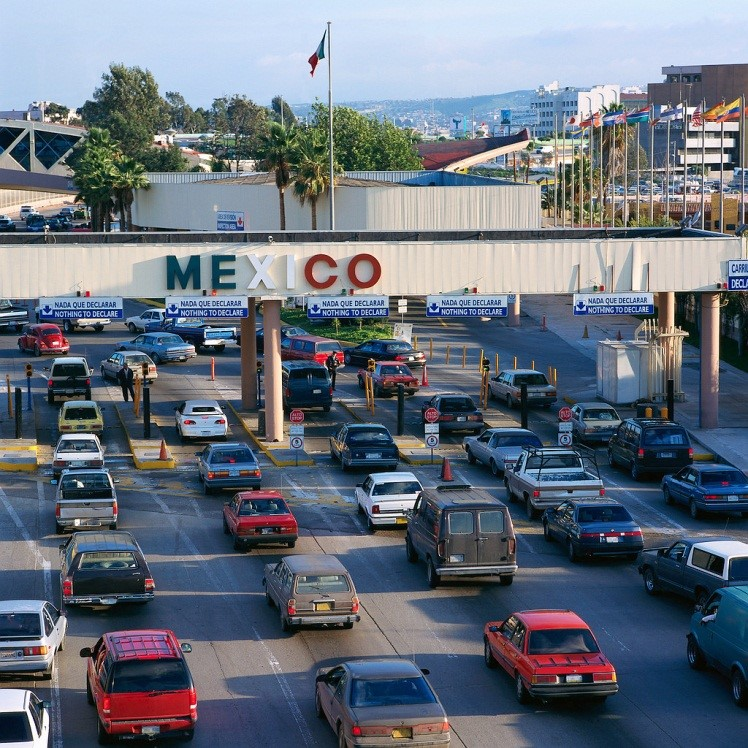
\includegraphics[width=0.7\linewidth]{./content/generalProvisions/contextDiagram}
\caption{Kontextdiagramm (Festlegung der Systemgrenze)}
\label{fig:contextDiagram}
\end{figure}


\note{This subsection should also describe how the system operates inside various constraints. For example, these constraints could include
\begin{enumerate}
\item System interfaces
\item User interfaces
\item Hardware interfaces
\item Software interfaces
\item Communications interfaces
\item Memory
\item Operations
\item Site adaptation requirements
\end{enumerate}
}
 
2.) Erstellung eines GUI für die erwähnte Applikation -> Verwendung von Qt \& C++. \\


\subsection{Produktfunktionen}
\note{Hier soll eine \textbf{Zusammenfassung} der Hauptfunktionen angeboten werden, welche das System erfüllen soll.}

\subsection{Benutzereigenschaften}
\note{Festlegung der Benutzer (Benutzergruppen), welche mit dem System arbeiten sollen, z.B. Routinebenutzer, Servicetechniker, Administrator. Dazu gehört auch die Definition der Kenntnisse und Erfahrungen der einzelnen Gruppen. Falls die funktionalen An-forderungen mittels Use Case – Diagrammen formuliert werden, dann entspricht dies den Actors, welche Personen repräsentieren.}

\subsection{Einschränkungen}
\note{This subsection of the SRS should provide a general description of any other items that will limit the developer's options. These include:

\begin{enumerate}
\item Regulatory policies:
\item Hardware limitations (e.g., signal timing requirements)
\item Interfaces to other applications
\item Parallel operation
\item Audit functions
\item Control functions
\item Higher-order language requirements: C++
\item Signal handshake protocols (e.g., XON-XOFF, ACK-NACK)
\item Reliability requirements:
\item Criticality of the application: Nein
\item Safety and security considerations: Nein
\end{enumerate}}

GUI-Programmierung mit Qt.
Angewiesen auf seine Vorlage. 


\subsection{Annahmen und Abhängigkeiten}
\note{This subsection of the SRS should list each of the factors that affect the requirements stated in the SRS. These factors are not design constraints on the system but are, rather, any changes to them that can affect the requirements in the SRS. For example, an assumption may be that a specific operating system will be available on the hardware designated for the software product. If, in fact, the operating system is not available, the SRS would then have to change accordingly.}

\subsection{Priorisierung der Anforderungen}
\note{Falls die Anforderungen unterschiedliche Prioritäten haben, bzw. einzelne Anforderungen erst in einer späteren Version implementiert werden sollen, dann kann das hier aufgelistet werden, z.B.
\begin{itemize}
\item Muss-Anforderung: dies ist eine Anforderung, welche für das System essentiell und unabdingbar ist, bzw. das System würde keinen Sinn ergeben, wenn diese Anforderung nicht implementiert wäre.
\item Soll-Anforderung: eine Soll-Anforderung ist nicht unabdingbar, trägt jedoch zur wesentlichen Verbesserung des Systems bei. Sie soll wenn möglich realisiert werden.
\item Wunsch-Anforderung (nice to have): diese Anforderung trägt zur Verbesserung des Systems bei, ist jedoch nicht unbedingt notwendig. Es ist ein Plus wenn diese Anforderung realisiert werden kann.
\end{itemize}
}

	\section{Externe Schnittstellen}
\label{sec:extIf}
\note{Ab diesem Abschnitt sollen alle Anforderungen in einem Detaillierungsgrad geschrieben sein, der es den Entwicklern ermöglicht, ein System zu entwerfen, welches diese Anforderungen erfüllt, d.h. der Entwickler sollte nun klar wissen, welche Anforderungen umgesetzt werden müssen. Ebenfalls müssen Testingenieure aufgrund dieser Anforderungen ihre (System-)Testfälle definieren können.

Jede Anforderung sollte eindeutig identifizierbar sein, beispielsweise durch eine eindeutige Nummer.

In diesem Kapitel sollen, allenfalls in Abschnitten organisiert, die folgenden Schnittstellen beschrieben werden:
\begin{itemize}
\item Benutzerschnittstellen : JA -> GUI
\item Hardwareschnittstellen: NEIN
\item Softwareschnittstellen: NEIN
\item Kommunikationsschnittstellen: NEIN
\end{itemize}
}

	\section{Funktionale Anforderungen}
\label{sec:funcReqs}
\note{Die funktionalen Anforderungen sind die wichtigsten Teile zur Beschreibung des Systems. Für die Beschreibung der funktionalen Anforderungen bieten sich Use Cases an, nicht nur für Software, sondern auch für das ganze System. Jeder Use Case beschreibt dabei eine Funktion. Im folgenden Raster ist vorgesehen, dass bei jedem Use Case auch nicht funktionale Anforderungen wie Antwortzeiten, etc. direkt beim Use Case stehen, falls diese zu dieser Funktion gehören.

Bei der Use Case Definition ist wichtig, dass die Granularität nicht zu fein gewählt wird. Allfällige Ausnahmefälle einer Funktion sollen beispielsweise in der Beschreibung des entsprechenden Use Cases geschehen und nicht allenfalls in einem "Unter-Use Case". 

Statt mittels Use Cases kann dieses Kapitel auch mit \textbf{Systemfunktion 1}, \textbf{Systemfunktion 2}, etc. gegliedert werden.}


\subsection{Überblick über die Systemfunktionen}
\note{Hier kommt ein Use Case Diagramm hinein, das alle Funktionen zeigt. Allenfalls genügt ein Link zum Abschnitt Systemübersicht.}


\subsection{Actors}
\note{Kurzbeschreibung der Actors.}


\subsection{Kurzbeschreibung der Use Cases}
\note{Jeder einzelne Use Case soll kurz beschrieben werden.}

Berechnung von 2 Widerstandswerten von einer bestimmten E-Serie, basierend auf einer Eingabe- und Ausgabespannung. 


\subsection{Spannungsteiler}
\note{Ist für jeden Use Case zu beschreiben. Die folgenden Unterkapitel sollen für jeden einzelnen Use Case vollständig vorhanden sein. Falls bei einem Abschnitt nichts zu schreiben ist, dann soll dies entsprechend vermerkt werden, z.B. falls ein Use Case keine Vorbedingungen braucht oder keine nicht-funktionalen Anforderungen vorhanden sind, kann bei diesem Abschnitt einfach das Wort "keine" stehen.}

Berechnung von 2 Widerstandswerten von einer bestimmten E-Serie, basierend auf einer Eingabe- und Ausgabespannung. 


\subsubsection{Vorbedingungen}
\note{Zustand des Systems bevor der Use Case eintritt, z.B. kann hier stehen, dass ein System erfolgreich initialisiert sein muss, damit diese Funktion ausgeführt werden kann.}

Keine Vorbedingungen.

\subsubsection{Nachbedingungen}
\note{Zustand des Systems nachdem der Use Case durchlaufen ist, z.B. kann hier bei einem Kalibrations-Use Case stehen, dass das System kalibriert oder allenfalls in einem Fehlerzustand ist.}

Widerstandswerte angegeben oder Fehlermeldung.

\subsubsection{Nicht-funktionale Anforderungen}
\note{Zusicherungen, die für Design und Realisierung wichtig sind, wie z.B. Antwortzeit, Häufigkeit, Priorität usw.}



\subsubsection{Hauptszenario}
\note{Beschreibung des Use Cases, ggf. gegliedert in Einzelpunkte. Beschrieben wird der Normalfall. Variationen werden mit Unterszenario-Nummer erwähnt (\textit{\textbf{[S-1]}} , \textit{\textbf{[S-2]}}, usw.) und separat als Unterszenarien beschrieben. Fehlerfälle werden mit Fehlerszenario-Nummern angegeben (\textit{\textbf{[E-1]}}, \textit{\textbf{[E-2]}}, usw.) und separat als Fehlerszenarien beschrieben.

Beispiele:
Falls gewünscht können zusätzliche Informationen erfasst werden \textit{\textbf{[S-1]}}.

Beim Einlesen der Daten können die Fehler \textit{\textbf{[E-1]}}, \textit{\textbf{[E-2]}} oder \textit{\textbf{[E-3]}} auftreten.}

\subsubsection{Unterszenarien}
\note{\textit{\textbf{[S-1]}} Zusatzinformationen erfassen

E1: Ohne Eingangs- und Ausgangsspannung können die Widerstandswerte nicht berechnet werden -> Fehlermeldung.
E2: Wenn kein max. oder min. Bereich angegeben wird, dann gibt es eine Fehlermeldung


\textit{\textbf{[S-2]}} ...}

\paragraph{\textit{\textbf{[S-1]}} Zusatzinformationen erfassen}
\paragraph{\textit{\textbf{[S-2]}} ...}

\subsubsection{Fehlerszenarien}
\note{\textit{\textbf{[E-1]}} Daten nicht verfügbar

\textit{\textbf{[E-2]}} Falsches Datenformat

\textit{\textbf{[E-3]}} ...}

\paragraph{\textit{\textbf{[E-1]}} Daten nicht verfügbar}
\paragraph{\textit{\textbf{[E-1]}} Falsches Datenformat}
\paragraph{\textit{\textbf{[E-2]}} ...}

\subsubsection{Regeln}
\note{Gültigkeits- und Validierungsregeln, Berechnungsformeln usw.}

\subsubsection{Anmerkungen}

\subsubsection{Beispiele}

	\section{Sonstige Anforderungen}
\label{sec:otherReqs}
\note{In diesesm Kapitel sollen alle bisher noch nicht spezifizierten Anforderungen, möglicherweise in Unterabschnitten, definiert werden, z.B.

\begin{itemize}
\item Leistungsanforderungen (Performance), die nicht direkt einer Systemfunktion zugeordnet werden konnten.
\item Entwurfseinschränkungen (Design Constraints): Anforderungen, welche die Entwickler bei der Wahl des Designs einschränken.
\item Qualitätsanforderungen wie Zuverlässigkeit, Verfügbarkeit, Sicherheit (Safety und Security, ist nicht dasselbe!)
\item Wartbarkeit
\item Portabilität
\item Logging und Tracing
\item Service und Support
\end{itemize}
}


	
	
% % % % % % % % % % % % % % % % % % % % % % % % % % % % % % % %
% ANHANG
% % % % % % % % % % % % % % % % % % % % % % % % % % % % % % % %
	\appendix
	
	%Nummerierung wieder auf roemisch umschalten
	\newpage
	
	\section{Referenzen}
	\label{anx:ref}
	% Do not repeat items covered in other documents or in a global project definitions and acronyms document
	\renewcommand{\refname}{} %kein Titel vor Literaturverzeichnis
	\vspace{-1.2cm}
	\bibliographystyle{plain} %Literatur durchnumerieren
	\bibliography{lit}
	\nocite{*} %Alle Literatur aufführen
	
\note{Do not repeat items covered in other documents or in a global project definitions and acronyms document}
	
\end{document}